% Options for packages loaded elsewhere
\PassOptionsToPackage{unicode}{hyperref}
\PassOptionsToPackage{hyphens}{url}
\PassOptionsToPackage{dvipsnames,svgnames,x11names}{xcolor}
%
\documentclass[
  letterpaper,
  DIV=11,
  numbers=noendperiod]{scrartcl}

\usepackage{amsmath,amssymb}
\usepackage{iftex}
\ifPDFTeX
  \usepackage[T1]{fontenc}
  \usepackage[utf8]{inputenc}
  \usepackage{textcomp} % provide euro and other symbols
\else % if luatex or xetex
  \usepackage{unicode-math}
  \defaultfontfeatures{Scale=MatchLowercase}
  \defaultfontfeatures[\rmfamily]{Ligatures=TeX,Scale=1}
\fi
\usepackage{lmodern}
\ifPDFTeX\else  
    % xetex/luatex font selection
\fi
% Use upquote if available, for straight quotes in verbatim environments
\IfFileExists{upquote.sty}{\usepackage{upquote}}{}
\IfFileExists{microtype.sty}{% use microtype if available
  \usepackage[]{microtype}
  \UseMicrotypeSet[protrusion]{basicmath} % disable protrusion for tt fonts
}{}
\makeatletter
\@ifundefined{KOMAClassName}{% if non-KOMA class
  \IfFileExists{parskip.sty}{%
    \usepackage{parskip}
  }{% else
    \setlength{\parindent}{0pt}
    \setlength{\parskip}{6pt plus 2pt minus 1pt}}
}{% if KOMA class
  \KOMAoptions{parskip=half}}
\makeatother
\usepackage{xcolor}
\setlength{\emergencystretch}{3em} % prevent overfull lines
\setcounter{secnumdepth}{5}
% Make \paragraph and \subparagraph free-standing
\ifx\paragraph\undefined\else
  \let\oldparagraph\paragraph
  \renewcommand{\paragraph}[1]{\oldparagraph{#1}\mbox{}}
\fi
\ifx\subparagraph\undefined\else
  \let\oldsubparagraph\subparagraph
  \renewcommand{\subparagraph}[1]{\oldsubparagraph{#1}\mbox{}}
\fi

\usepackage{color}
\usepackage{fancyvrb}
\newcommand{\VerbBar}{|}
\newcommand{\VERB}{\Verb[commandchars=\\\{\}]}
\DefineVerbatimEnvironment{Highlighting}{Verbatim}{commandchars=\\\{\}}
% Add ',fontsize=\small' for more characters per line
\usepackage{framed}
\definecolor{shadecolor}{RGB}{241,243,245}
\newenvironment{Shaded}{\begin{snugshade}}{\end{snugshade}}
\newcommand{\AlertTok}[1]{\textcolor[rgb]{0.68,0.00,0.00}{#1}}
\newcommand{\AnnotationTok}[1]{\textcolor[rgb]{0.37,0.37,0.37}{#1}}
\newcommand{\AttributeTok}[1]{\textcolor[rgb]{0.40,0.45,0.13}{#1}}
\newcommand{\BaseNTok}[1]{\textcolor[rgb]{0.68,0.00,0.00}{#1}}
\newcommand{\BuiltInTok}[1]{\textcolor[rgb]{0.00,0.23,0.31}{#1}}
\newcommand{\CharTok}[1]{\textcolor[rgb]{0.13,0.47,0.30}{#1}}
\newcommand{\CommentTok}[1]{\textcolor[rgb]{0.37,0.37,0.37}{#1}}
\newcommand{\CommentVarTok}[1]{\textcolor[rgb]{0.37,0.37,0.37}{\textit{#1}}}
\newcommand{\ConstantTok}[1]{\textcolor[rgb]{0.56,0.35,0.01}{#1}}
\newcommand{\ControlFlowTok}[1]{\textcolor[rgb]{0.00,0.23,0.31}{#1}}
\newcommand{\DataTypeTok}[1]{\textcolor[rgb]{0.68,0.00,0.00}{#1}}
\newcommand{\DecValTok}[1]{\textcolor[rgb]{0.68,0.00,0.00}{#1}}
\newcommand{\DocumentationTok}[1]{\textcolor[rgb]{0.37,0.37,0.37}{\textit{#1}}}
\newcommand{\ErrorTok}[1]{\textcolor[rgb]{0.68,0.00,0.00}{#1}}
\newcommand{\ExtensionTok}[1]{\textcolor[rgb]{0.00,0.23,0.31}{#1}}
\newcommand{\FloatTok}[1]{\textcolor[rgb]{0.68,0.00,0.00}{#1}}
\newcommand{\FunctionTok}[1]{\textcolor[rgb]{0.28,0.35,0.67}{#1}}
\newcommand{\ImportTok}[1]{\textcolor[rgb]{0.00,0.46,0.62}{#1}}
\newcommand{\InformationTok}[1]{\textcolor[rgb]{0.37,0.37,0.37}{#1}}
\newcommand{\KeywordTok}[1]{\textcolor[rgb]{0.00,0.23,0.31}{#1}}
\newcommand{\NormalTok}[1]{\textcolor[rgb]{0.00,0.23,0.31}{#1}}
\newcommand{\OperatorTok}[1]{\textcolor[rgb]{0.37,0.37,0.37}{#1}}
\newcommand{\OtherTok}[1]{\textcolor[rgb]{0.00,0.23,0.31}{#1}}
\newcommand{\PreprocessorTok}[1]{\textcolor[rgb]{0.68,0.00,0.00}{#1}}
\newcommand{\RegionMarkerTok}[1]{\textcolor[rgb]{0.00,0.23,0.31}{#1}}
\newcommand{\SpecialCharTok}[1]{\textcolor[rgb]{0.37,0.37,0.37}{#1}}
\newcommand{\SpecialStringTok}[1]{\textcolor[rgb]{0.13,0.47,0.30}{#1}}
\newcommand{\StringTok}[1]{\textcolor[rgb]{0.13,0.47,0.30}{#1}}
\newcommand{\VariableTok}[1]{\textcolor[rgb]{0.07,0.07,0.07}{#1}}
\newcommand{\VerbatimStringTok}[1]{\textcolor[rgb]{0.13,0.47,0.30}{#1}}
\newcommand{\WarningTok}[1]{\textcolor[rgb]{0.37,0.37,0.37}{\textit{#1}}}

\providecommand{\tightlist}{%
  \setlength{\itemsep}{0pt}\setlength{\parskip}{0pt}}\usepackage{longtable,booktabs,array}
\usepackage{calc} % for calculating minipage widths
% Correct order of tables after \paragraph or \subparagraph
\usepackage{etoolbox}
\makeatletter
\patchcmd\longtable{\par}{\if@noskipsec\mbox{}\fi\par}{}{}
\makeatother
% Allow footnotes in longtable head/foot
\IfFileExists{footnotehyper.sty}{\usepackage{footnotehyper}}{\usepackage{footnote}}
\makesavenoteenv{longtable}
\usepackage{graphicx}
\makeatletter
\def\maxwidth{\ifdim\Gin@nat@width>\linewidth\linewidth\else\Gin@nat@width\fi}
\def\maxheight{\ifdim\Gin@nat@height>\textheight\textheight\else\Gin@nat@height\fi}
\makeatother
% Scale images if necessary, so that they will not overflow the page
% margins by default, and it is still possible to overwrite the defaults
% using explicit options in \includegraphics[width, height, ...]{}
\setkeys{Gin}{width=\maxwidth,height=\maxheight,keepaspectratio}
% Set default figure placement to htbp
\makeatletter
\def\fps@figure{htbp}
\makeatother
\newlength{\cslhangindent}
\setlength{\cslhangindent}{1.5em}
\newlength{\csllabelwidth}
\setlength{\csllabelwidth}{3em}
\newlength{\cslentryspacingunit} % times entry-spacing
\setlength{\cslentryspacingunit}{\parskip}
\newenvironment{CSLReferences}[2] % #1 hanging-ident, #2 entry spacing
 {% don't indent paragraphs
  \setlength{\parindent}{0pt}
  % turn on hanging indent if param 1 is 1
  \ifodd #1
  \let\oldpar\par
  \def\par{\hangindent=\cslhangindent\oldpar}
  \fi
  % set entry spacing
  \setlength{\parskip}{#2\cslentryspacingunit}
 }%
 {}
\usepackage{calc}
\newcommand{\CSLBlock}[1]{#1\hfill\break}
\newcommand{\CSLLeftMargin}[1]{\parbox[t]{\csllabelwidth}{#1}}
\newcommand{\CSLRightInline}[1]{\parbox[t]{\linewidth - \csllabelwidth}{#1}\break}
\newcommand{\CSLIndent}[1]{\hspace{\cslhangindent}#1}

\KOMAoption{captions}{tableheading}
\makeatletter
\makeatother
\makeatletter
\makeatother
\makeatletter
\@ifpackageloaded{caption}{}{\usepackage{caption}}
\AtBeginDocument{%
\ifdefined\contentsname
  \renewcommand*\contentsname{Table of contents}
\else
  \newcommand\contentsname{Table of contents}
\fi
\ifdefined\listfigurename
  \renewcommand*\listfigurename{List of Figures}
\else
  \newcommand\listfigurename{List of Figures}
\fi
\ifdefined\listtablename
  \renewcommand*\listtablename{List of Tables}
\else
  \newcommand\listtablename{List of Tables}
\fi
\ifdefined\figurename
  \renewcommand*\figurename{Figure}
\else
  \newcommand\figurename{Figure}
\fi
\ifdefined\tablename
  \renewcommand*\tablename{Table}
\else
  \newcommand\tablename{Table}
\fi
}
\@ifpackageloaded{float}{}{\usepackage{float}}
\floatstyle{ruled}
\@ifundefined{c@chapter}{\newfloat{codelisting}{h}{lop}}{\newfloat{codelisting}{h}{lop}[chapter]}
\floatname{codelisting}{Listing}
\newcommand*\listoflistings{\listof{codelisting}{List of Listings}}
\makeatother
\makeatletter
\@ifpackageloaded{caption}{}{\usepackage{caption}}
\@ifpackageloaded{subcaption}{}{\usepackage{subcaption}}
\makeatother
\makeatletter
\@ifpackageloaded{tcolorbox}{}{\usepackage[skins,breakable]{tcolorbox}}
\makeatother
\makeatletter
\@ifundefined{shadecolor}{\definecolor{shadecolor}{rgb}{.97, .97, .97}}
\makeatother
\makeatletter
\makeatother
\makeatletter
\makeatother
\ifLuaTeX
  \usepackage{selnolig}  % disable illegal ligatures
\fi
\IfFileExists{bookmark.sty}{\usepackage{bookmark}}{\usepackage{hyperref}}
\IfFileExists{xurl.sty}{\usepackage{xurl}}{} % add URL line breaks if available
\urlstyle{same} % disable monospaced font for URLs
\hypersetup{
  pdftitle={Network simplification: application to the visualisation of transport networks},
  colorlinks=true,
  linkcolor={blue},
  filecolor={Maroon},
  citecolor={Blue},
  urlcolor={Blue},
  pdfcreator={LaTeX via pandoc}}

\title{Network simplification: application to the visualisation of
transport networks}
\author{}
\date{}

\begin{document}
\maketitle
\ifdefined\Shaded\renewenvironment{Shaded}{\begin{tcolorbox}[sharp corners, borderline west={3pt}{0pt}{shadecolor}, frame hidden, enhanced, boxrule=0pt, breakable, interior hidden]}{\end{tcolorbox}}\fi

\hypertarget{reproducibility}{%
\section*{Reproducibility}\label{reproducibility}}
\addcontentsline{toc}{section}{Reproducibility}

To reproduce this paper you need \texttt{quarto} installed and the
Elsevier extension which can be installed as follows:

\begin{Shaded}
\begin{Highlighting}[]
\ExtensionTok{quarto}\NormalTok{ add quarto{-}journals/elsevier}
\end{Highlighting}
\end{Shaded}

To write the paper we recommend using the Quarto extension for VS Code.
You can go into the visual editor with the following shortcut:

\begin{verbatim}
Ctrl+Shift+F4
\end{verbatim}

You can then add citations and other elements of academic writing.

\hypertarget{abstract}{%
\section*{Abstract}\label{abstract}}
\addcontentsline{toc}{section}{Abstract}

\hypertarget{introduction}{%
\section{Introduction}\label{introduction}}

Datasets representing route networks are central to transport planning.
Unlike other key types of data used in transport planning, route
networks are both a key input \emph{and} key output. Origin-destination,
GPS, and remote sensing imagery datasets are all key inputs but rarely
feature as outputs of transport models. Global and local estimates of
costs and benefits associated with changes to transport systems,
geographic outputs at regional, local and corridor level, and
visualisation of agents on the system are common outputs. However, route
network datasets are ubiquitous as both transport model inputs
(typically representing road networks) outputs (typically with model
outputs such as flow per time of day).\footnote{See the
  \href{https://sumo.dlr.de/docs/Simulation/Output/index.html}{online
  documentation} of the SUMO traffic simulation tool for an example of
  the wide range of data formats that transport datasets can output.}

This raises the question, what are transport network datasets? The
intuitive definition is that route network datasets are digital
representations of footpaths, cycleways, highways and other ways along
which people and goods can travel. More formally, transport network
datasets must contain, at a minimum, geographic information on the
coordinates of vertices (points along ways) and edges (the straight
lines between vertices representing ways). Usually they also contain
attributes associated with these ways. File formats for representing
them include Transportation Network Test Problem (TNTP and stored as a
series of \texttt{.tntp} plain text files, examples of which can be
found in
\href{https://github.com/bstabler/TransportationNetworks}{github.com/bstabler/TransportationNetworks}),
\texttt{.DAT} files used by the proprietary SATURN transport modelling
system and XML-based \texttt{.osm} or \texttt{.pbf} files that encode
OpenStreetMap data.

A more recent approach is to represent transport networks in standard
geographic file formats. In this approach, used in the present paper,
transport networks are represented as a series of non-overlapping
linestrings, with attributes such as way type and flow. Making transport
datasets compliant with the `simple features' geographic data
specification in this way has many advantages compared with the
proliferation of formats used by proprietary software, enabling more
easier sharing of datasets between people and programs. The simple
features standard is formalised by the International Organization for
Standardization in \href{https://www.iso.org/standard/40114.html}{ISO
19125-1:2004} and implemented in a wide range of file formats such as
ESRIs shapefile, GeoJSON, and the open standard for geographic data,
GeoPackage. For ease of data sharing, we share transport networks used
in this paper as plain text GeoJSON files.

Much research has focussed on generating and modelling transport network
datasets. This is unsurprising given the importance of transport
networks as inputs and outputs of transport models. Much has been
written about network `cleaning' and simplification as a pre-processing
step in transport modelling. However, there has been relatively little
research into transport network visualisation, despite the importance of
visualisation to enable more people to understand transport models, for
informing policies and prioritising investment in transport planning.

Morgan and Lovelace (2020) presented methods for combining multiple
overlapping routes into a single route network with non-overlapping
linestrings for visualisation, implemented in the function
\texttt{overline()}. The approach takes overlapping linestrings
representing multiple routes and combines them into a single network
with non-overlapping linestrings. The approach has been used to
visualise large transport networks, informing investment decisions in
transport planning internationally. However, the `overline' approach,
without further processing, has limitations:

\begin{itemize}
\tightlist
\item
  It does not remove redundant vertices, which can lead to large file
  sizes and slow rendering.
\item
  It does not remove redundant edges, which can lead to visual
  artefacts.
\item
  Parallel ways that are part of the same corridor are not merged into a
  single way, resulting in outputs that are difficult to interpret.
\end{itemize}

The final point is most relevant to the present paper. An example of the
issue is shown in Figure~\ref{fig-pct} from the Propensity to Cycle Tool
for England (PCT), with segment values representing daily commuter
cycling potential flows (Lovelace et al. 2017). The left panel shows
Otley Road with a flow value of 818 (Figure~\ref{fig-otley-road}). The
right panel, by contrast, shows three parallel ways parallel to Armley
Road with flow values of 515 (shown), 288 and 47 (values not shown)
(Figure~\ref{fig-armley-road}). Although this section of Armley road has
a higher cycling potential than the section of Otley Road shown (515 +
288 + 47 \textgreater{} 818), this is not clear from the visualisation.

\begin{figure}

\begin{minipage}[t]{0.50\linewidth}

{\centering 

\raisebox{-\height}{

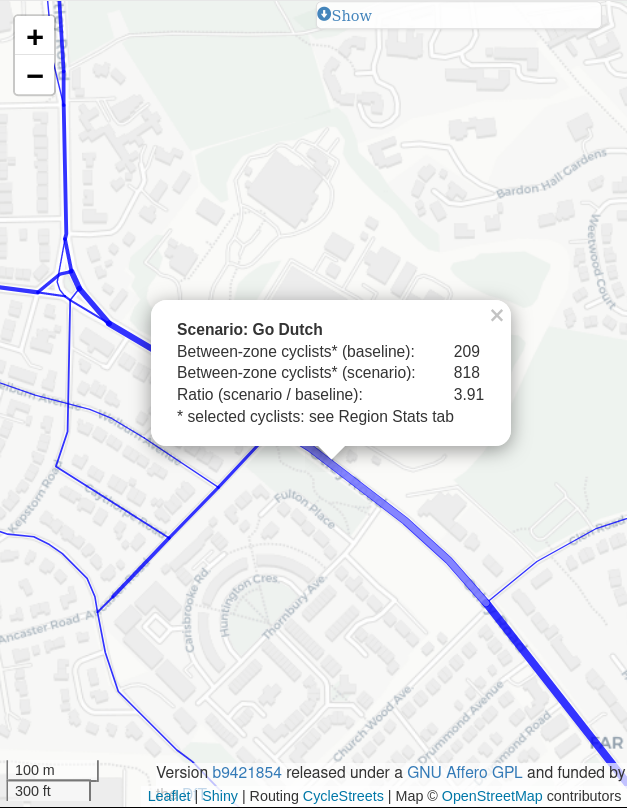
\includegraphics{images/otley-road-narrow.png}

}

}

\subcaption{\label{fig-otley-road}}
\end{minipage}%
%
\begin{minipage}[t]{0.50\linewidth}

{\centering 

\raisebox{-\height}{

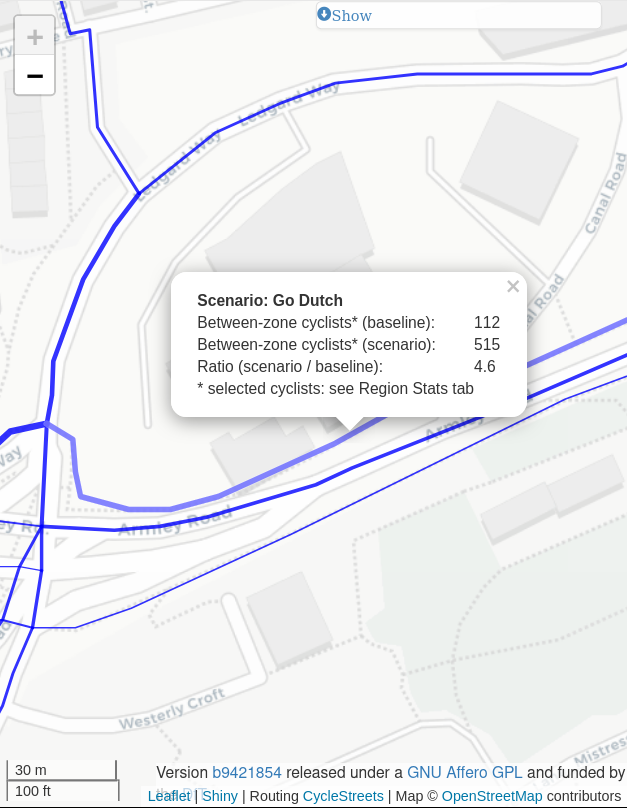
\includegraphics{images/armley-road-narrow.png}

}

}

\subcaption{\label{fig-armley-road}}
\end{minipage}%

\caption{\label{fig-pct}Illustration of issues associated with route
network-level results containing multiple parallel ways on the same
corridor: it is not clear from the visualisation that the corridor shown
in the right hand figure has greater flow than the corridor shown in the
left. Source: open access Propensity to Cycle Tool results available at
www.pct.bike.}

\end{figure}

A subsequent step described in the paper is to post-process the
geographic representation of the transport network into a raster image,
which can be used to visualise the network. The `rasterisation' stage
can tackle some of the issues associated with multiple parallel ways,
but introduces new issues, as shown in Figure~\ref{fig-rasterisation}.

\begin{figure}

\begin{minipage}[t]{0.50\linewidth}

{\centering 

\raisebox{-\height}{

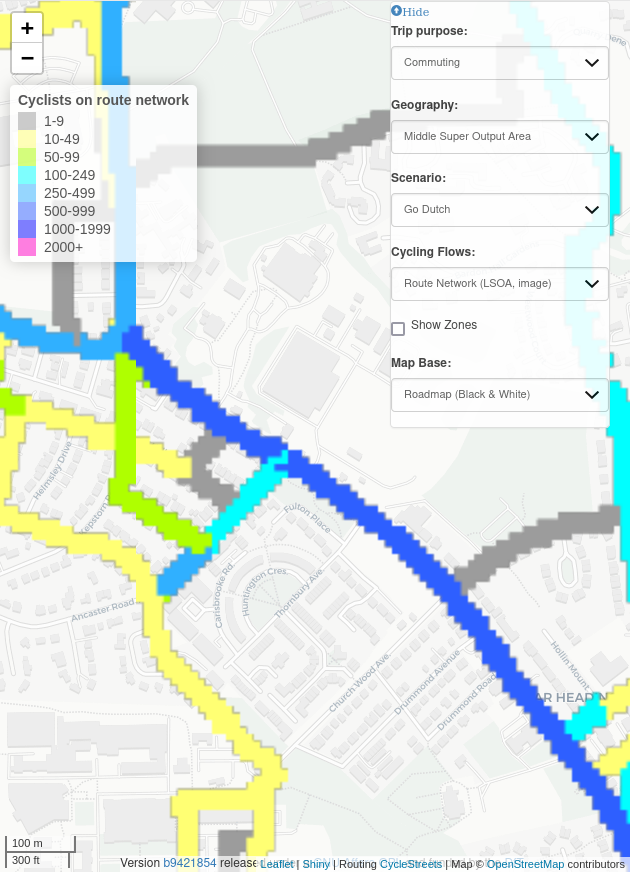
\includegraphics{images/otley-road-raster.png}

}

}

\subcaption{\label{fig-otley-road-raster}}
\end{minipage}%
%
\begin{minipage}[t]{0.50\linewidth}

{\centering 

\raisebox{-\height}{

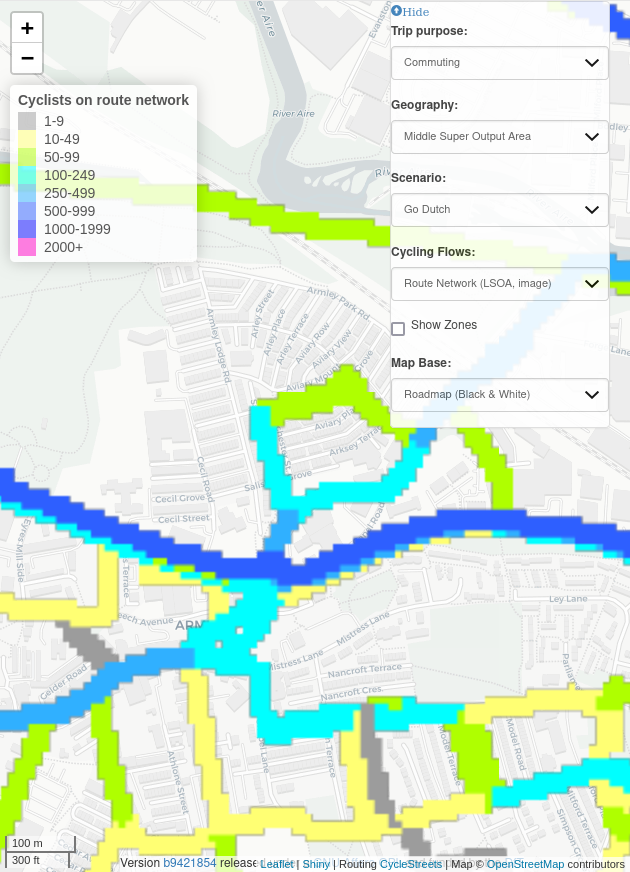
\includegraphics{images/armley-road-raster.png}

}

}

\subcaption{\label{fig-armley-road-raster}}
\end{minipage}%

\caption{\label{fig-rasterisation}Rasterised network results for the
same corridors shown in Figure~\ref{fig-pct}. Note the visual artefacts
such as `staircase' effects and overlapping values resulting from
parallel lines along Armley Road (right panel). Source: open access
Propensity to Cycle Tool results available at www.pct.bike.}

\end{figure}

The methods presented in this paper are designed to take a complex
network as an input and output a simplified network, while preserving
the spatial structure of the network and relevant attribures. By
reducing duplicated parallel lines and other intricacies, the outputs
can enable easier-to-interpret visualisations of transport behaviour on
the network patterns and behaviors.

The aim of this paper is to outline approaches for visualising transport
networks that address the issues associated with multiple parallel ways.
Furthermore we present solutions, implemented with open source software
for reproducible and scalable results, to support better visualisation
of transport networks for more evidence-based and sustainable transport
planning.

Section~\ref{sec-methods} describes the input datasets and methods used
to generate the results presented in this paper.
Section~\ref{sec-results} presents the results, illustrated by network
maps of the example datasets. Finally, Section~\ref{sec-discussion}
discusses the results and outlines future work.

\hypertarget{data}{%
\section{Data}\label{data}}

\hypertarget{sec-methods}{%
\section{Methods}\label{sec-methods}}

Two fundamental approaches to simplifying transport networks are:

\begin{itemize}
\tightlist
\item
  Simplifying the geometry of the network, by removing redundant
  vertices and edges and/or by merging parallel ways and \emph{then}
  merging the attributes of the original network onto the simplified
  network.
\item
  Iteratively removing edges and updating the attributes of the
  remaining edges by routing through the network.
\end{itemize}

In this paper we will focus on the former approach, which assumes that a
simplified geographic representation of the network is available.

\hypertarget{geometry-simplification}{%
\subsection{Geometry simplification}\label{geometry-simplification}}

A prerequisite of simple networks is simple geometries.

\hypertarget{topology-preserving-simplification}{%
\subsubsection{Topology-preserving
simplification}\label{topology-preserving-simplification}}

Topology-preserving simplification reduces the number of vertices in a
linestring while preserving the topology of the network. As shown in top
panel of Figure~\ref{fig-topology-preserving}, topology-preserving
simplication \emph{can} reduce the number of edges, but fails to merge
parallel lines in complex geometries, as shown in the the bottom panel
in Figure~\ref{fig-topology-preserving}.

\begin{figure}

\begin{minipage}[t]{\linewidth}

{\centering 

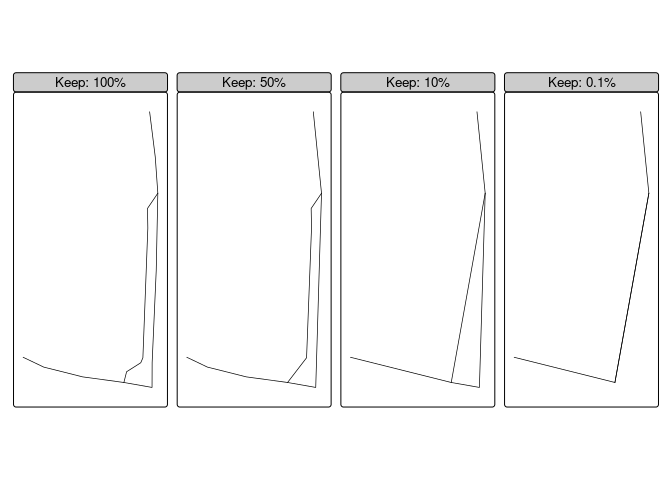
\includegraphics{paper_files/figure-pdf/unnamed-chunk-3-1.pdf}

}

\end{minipage}%
\newline
\begin{minipage}[t]{\linewidth}

{\centering 

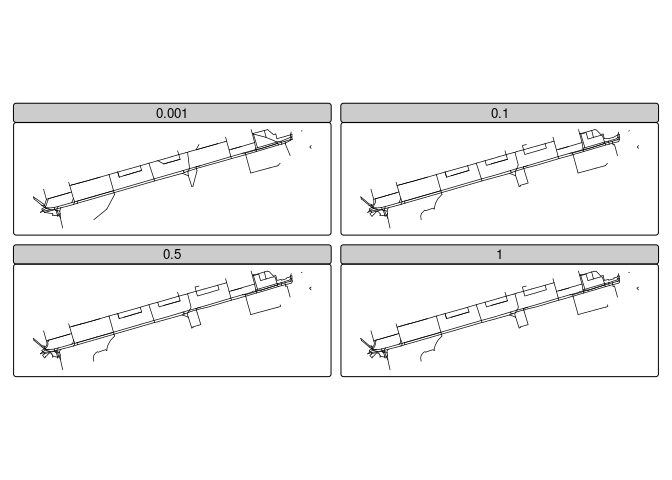
\includegraphics{paper_files/figure-pdf/unnamed-chunk-4-1.pdf}

}

\end{minipage}%

\caption{\label{fig-topology-preserving}Illustration of
topology-preserving simplification, using the \texttt{mapshaper}
JavaScript package. The \% values represent the ``percentage of
removable points to retain'' argument values used in the simplification
process.}

\end{figure}

The graphic below shows a 2 panel plot showing simplification with the
\texttt{consolidate\_intersections} function from the \texttt{osmnx}
Python package.

\begin{figure}

\begin{minipage}[t]{0.50\linewidth}

{\centering 

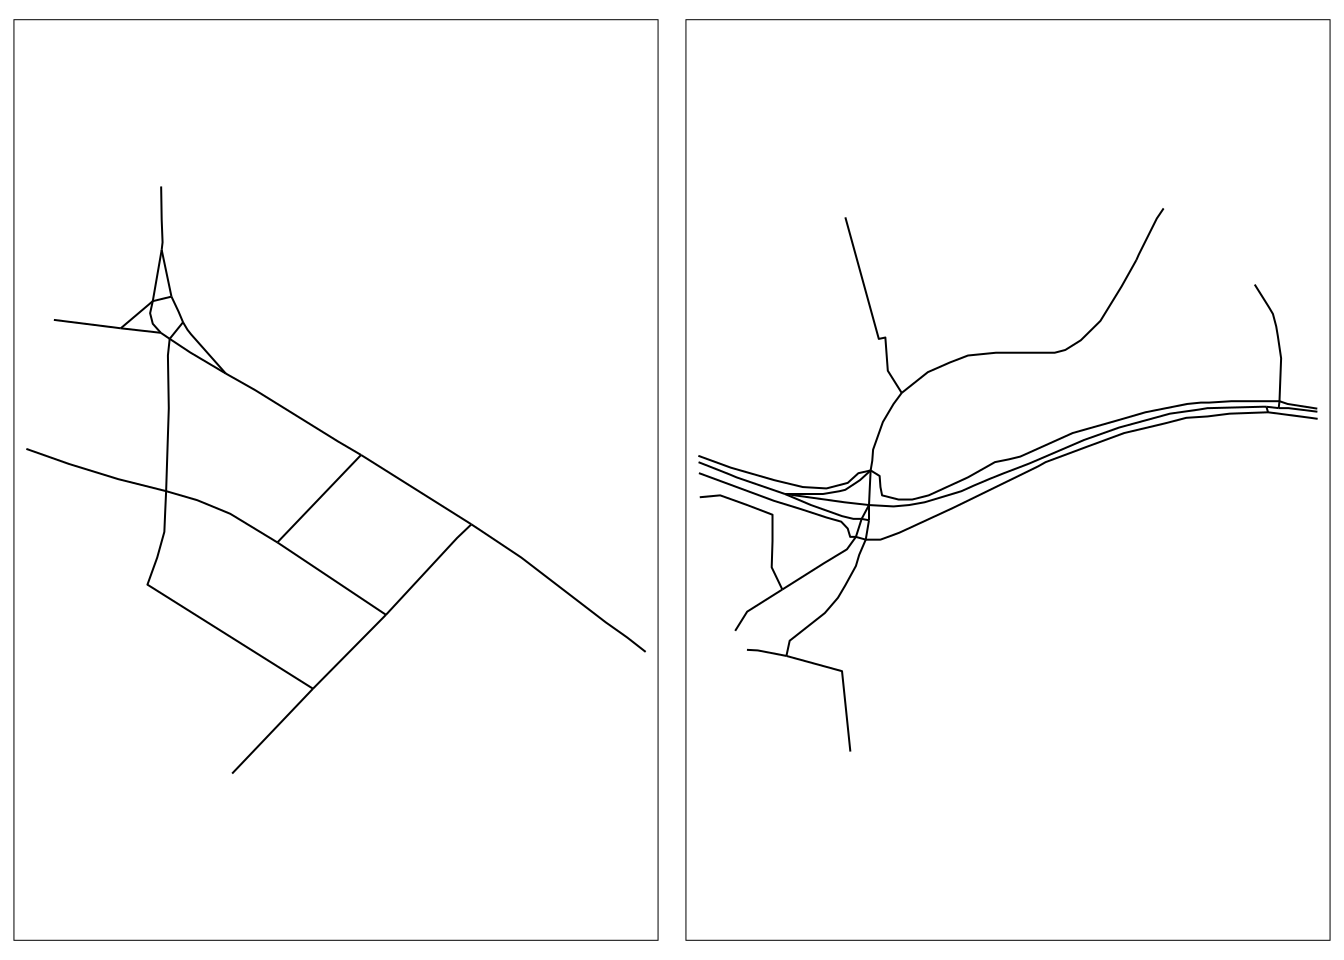
\includegraphics{paper_files/figure-pdf/unnamed-chunk-5-1.pdf}

}

\end{minipage}%
%
\begin{minipage}[t]{0.50\linewidth}

{\centering 

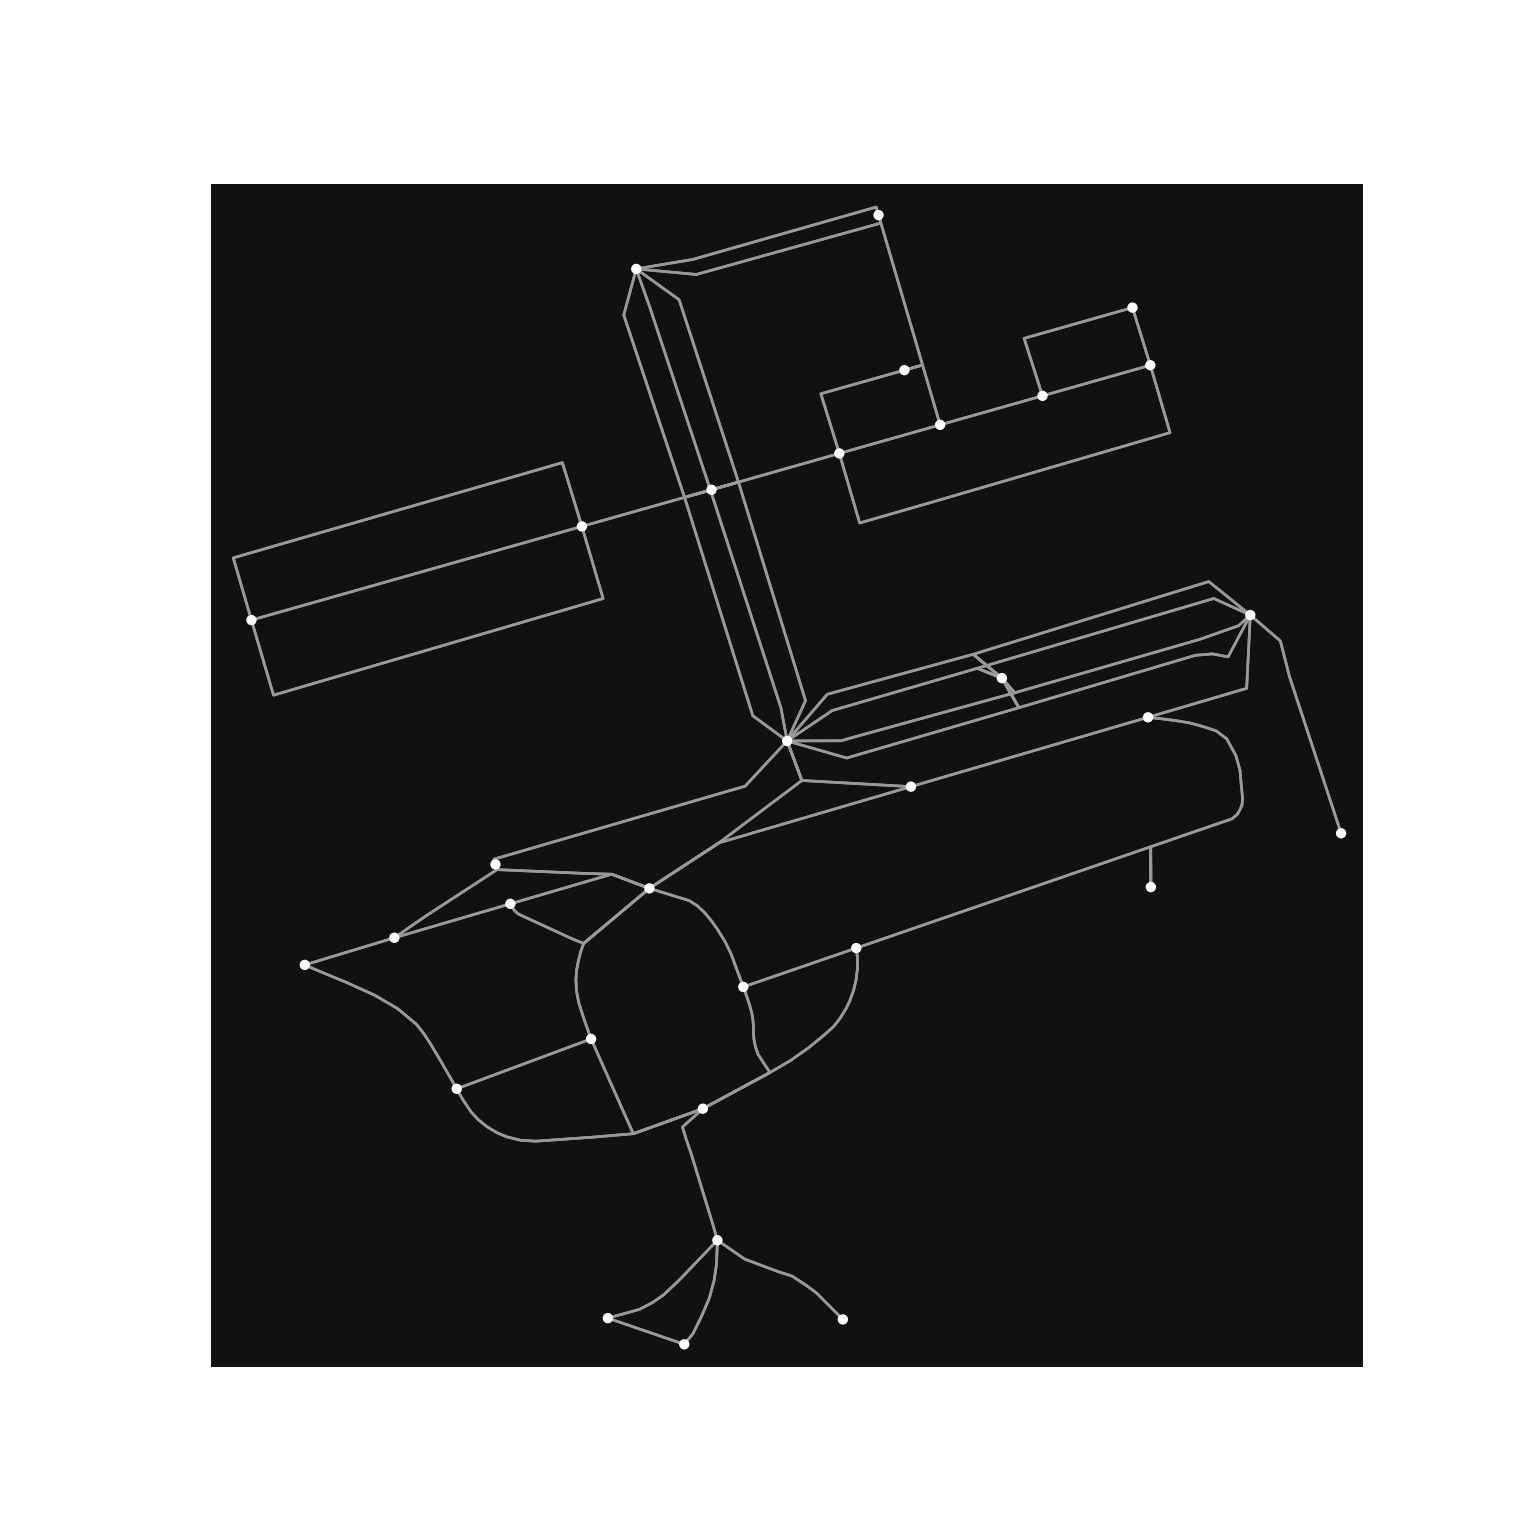
\includegraphics{paper_files/figure-pdf/unnamed-chunk-6-3.pdf}

}

\end{minipage}%

\caption{\label{fig-osmnx-consolidate-intersections}Illustration of
consolidation of intersections, with the
\texttt{consolidate\_intersections} function from the \texttt{osmnx}
Python package.}

\end{figure}

\hypertarget{simplification-with-parallel-edge-removal}{%
\subsubsection{Simplification with parallel edge
removal}\label{simplification-with-parallel-edge-removal}}

A more aggressive approach is to simplify and alter network topology in
a single step, ``through the removal of duplicate or parallel edges, and
combining simply-connected nodes'' (Deakin 2023).

\hypertarget{merging-simple-and-detailed-networks}{%
\subsection{Merging simple and detailed
networks}\label{merging-simple-and-detailed-networks}}

After you have a simplified version of the network, from any source, the
next step is merging the attributes.

\hypertarget{sec-results}{%
\section{Results}\label{sec-results}}

\hypertarget{sec-discussion}{%
\section{Discussion}\label{sec-discussion}}

\hypertarget{references}{%
\section{References}\label{references}}

\hypertarget{refs}{}
\begin{CSLReferences}{1}{0}
\leavevmode\vadjust pre{\hypertarget{ref-deakin2023}{}}%
Deakin, Will. 2023. \emph{Transport Network Simplification Through
Network Disaggregation and Reassembly of OpenStreet Map (OSM) Networks}.
\url{https://github.com/anisotropi4/graph}.

\leavevmode\vadjust pre{\hypertarget{ref-lovelace2017}{}}%
Lovelace, Robin, Anna Goodman, Rachel Aldred, Nikolai Berkoff, Ali
Abbas, and James Woodcock. 2017. {``The Propensity to Cycle Tool: An
Open Source Online System for Sustainable Transport Planning.''}
\emph{Journal of Transport and Land Use} 10 (1).
\url{https://doi.org/10.5198/jtlu.2016.862}.

\leavevmode\vadjust pre{\hypertarget{ref-morgan2020}{}}%
Morgan, Malcolm, and Robin Lovelace. 2020. {``Travel Flow Aggregation:
Nationally Scalable Methods for Interactive and Online Visualisation of
Transport Behaviour at the Road Network Level.''} \emph{Environment \&
Planning B: Planning \& Design}, July.
\url{https://doi.org/10.1177/2399808320942779}.

\end{CSLReferences}



\end{document}
